\subsection{U-Net predictions for treatment prediction}
With the new segmentations produced by the U-Net model, treatment prediction was attempted again. This time the same 1D ResNet model was used, but training consisted of 70 epochs with a learning rate of $10^{-4}$ and with $0.01$ weight decay. Cross entropy was used as loss function and Adam was used for optimization.

\begin{table}[H]
	\hspace{-2.7cm}
	\begin{tabular}{|c|c|c|c|c|c|c|c|c|c|c|c|c|c|c|c|c|c|c|c|c|c|c|c|c|c|}
		\hline
		Idx&1
		&7
		&8
		&14
		&15
		&16
		&17
		&18
		&19
		&20
		&21
		&22
		&23
		&24
		&25
		&26
		&27
		&28
		&29
		&30
		&31
		&32
		&33
		&34
		&35\\\hline\hline
		Predictions&0
		&2
		&1
		&2
		&2
		&2
		&1
		&1
		&1
		&1
		&1
		&2
		&1
		&1
		&1
		&0
		&1
		&1
		&1
		&0
		&2
		&0
		&2
		&2
		&2\\\hline
		True&1
		&3
		&3
		&4
		&2
		&2
		&2
		&1
		&1
		&2
		&2
		&2
		&2
		&1
		&0
		&0
		&0
		&1
		&0
		&0
		&0
		&0
		&2
		&2
		&2\\\hline
	\end{tabular}
	\caption{Training a model only on the predicted U-Net segmentations, we find the following treatment predictions and true treatments shown for each video. The treatment classes are: 0 being 'healthy', 1 being 'local 5-ASA', 2 being 'Oral steroid', 3 being 'IV steroid' and 4 being 'oral 5-ASA'.}
	\label{unetPredsTreatmentTable}
\end{table}

\begin{figure}[H]
	\centering
	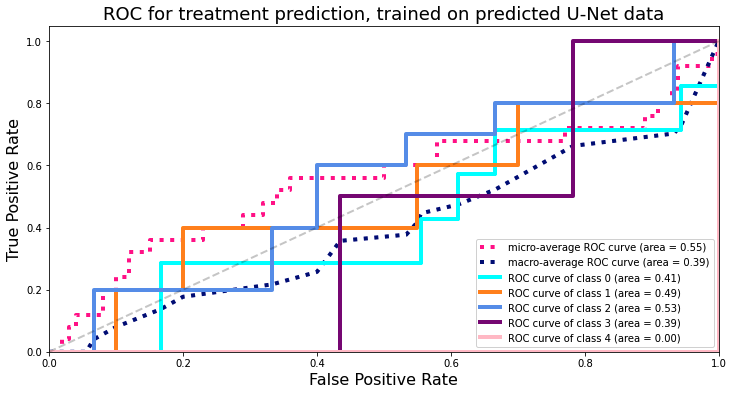
\includegraphics[width=0.85\linewidth]{Materials/Results/UNet/UNetROC1}
	\caption{ROC curves and area under the curve for the five binary 'one-vs-rest' classifiers along with micro- and macro-averages. Training was performed only on predicted segmentations.}
	\label{rocunetpreds}
\end{figure}
In \autoref{unetPredsTreatmentTable} we see the predicted treatments along the true prescribed treatment when we train only on the predicted segmentations from the U-Net model. In contrast to the previous results we now see predictions of classes $0, 1$ and $2$, where we previously did not see any predictions of treatment $1$. We also see an improvement in accuracy as we now have $52\%$.\\
Five binary 'one-vs-rest' classifiers were also trained for these predictions, and they were again trained using the same parameters as the multi class classifier. In \autoref{rocunetpreds} we see ROC curves for these binary classifiers, and we note the area under the curves being either $0.5$ or $0.4$ for all classes except class 4 which has $0.0$, which is significantly worse than for the previous treatment predictions.

When we include the true segmentations to the training data and repeat the experiment with the same parameters, we find the results seen in \autoref{unetPredsTrueTreatmentTable}. Here we again see the model predicting three classes, however, the accuracy drastically drops to $20\%$.

\begin{table}[H]
	\hspace{-2.7cm}
	\begin{tabular}{|c|c|c|c|c|c|c|c|c|c|c|c|c|c|c|c|c|c|c|c|c|c|c|c|c|c|}
		\hline
		Idx&1
		&7
		&8
		&14
		&15
		&16
		&17
		&18
		&19
		&20
		&21
		&22
		&23
		&24
		&25
		&26
		&27
		&28
		&29
		&30
		&31
		&32
		&33
		&34
		&35\\\hline\hline
		Predictions&2
		&2
		&2
		&2
		&1
		&1
		&1
		&2
		&2
		&2
		&1
		&1
		&2
		&2
		&1
		&2
		&2
		&2
		&2
		&2
		&1
		&0
		&2
		&1
		&2\\\hline
		True&1
		&3
		&3
		&4
		&2
		&2
		&2
		&1
		&1
		&2
		&2
		&2
		&2
		&1
		&0
		&0
		&0
		&1
		&0
		&0
		&0
		&0
		&2
		&2
		&2\\\hline
	\end{tabular}
	\caption{Training a model on the predicted U-Net segmentations and the true segmentations, we find the following treatment predictions and true treatments shown for each video. The treatment classes are: 0 being 'healthy', 1 being 'local 5-ASA', 2 being 'Oral steroid', 3 being 'IV steroid' and 4 being 'oral 5-ASA'.}
	\label{unetPredsTrueTreatmentTable}
\end{table}

In \autoref{rocunetpredstrue} we see the ROC curves when we add the true segmentations. Here, however, we see the area under the curve for class $0$ being a fair bit above $0.5$, indicating predictions for class $0$ are not random, while classes $1$ and $2$ are slightly above $0.5$. 

\begin{figure}[H]
	\centering
	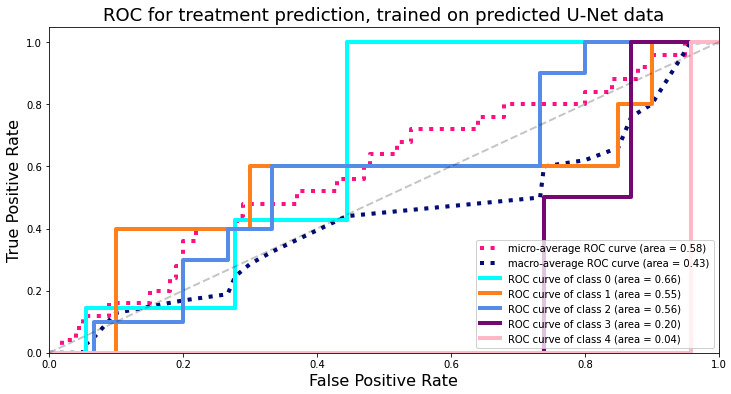
\includegraphics[width=0.85\linewidth]{Materials/Results/UNet/UNetROC2}
	\caption{ROC curves and area under the curve for the five binary 'one-vs-rest' classifiers along with micro- and macro-averages. Training was performed only on predicted segmentations.}
	\label{rocunetpredstrue}
\end{figure}